\subsection{Experimental Setup}

All benchmarks were run on a single machine: Windows~11 Home
(Version~10.0.26200, Build~26200), Intel Core Ultra~7~258V (8~cores,
x86-64), 32\,GB RAM, Rust~1.85. Each prover invocation was given a
1{,}000\,ms wall-clock timeout, a recursive search-depth limit of 128, and
a fresh-fallback budget of one term per quantified occurrence. For the TPTP
and FOLIO datasets a step limit of 10{,}000 rule applications was also
imposed. For the synthetic dataset the step limit was set to effectively
unlimited (10$^{11}$), with the wall-clock timeout as the sole binding
resource constraint; an initial run with 10{,}000 steps produced too few
decisions on synthetic problems to be informative, so the limit was
raised. Problems whose non-comment biconditional
($\Leftrightarrow$) count exceeds six are skipped before parsing; this cap
prevents large biconditional chains from consuming proof-search resources
disproportionate to the rest of the benchmark. Results were persisted to SQLite databases; the analysis pipeline
(Python~3.12 with \texttt{pandas} and \texttt{matplotlib}) loads all
results directly, as each database contains exactly one run per engine at
identical parameter settings.

\subsection{Datasets}

Three datasets are used, covering standard ATP benchmarks,
natural-language-derived problems, and synthetic controlled problems.

\subsubsection{TPTP.}
Two subsets of the TPTP problem library~\cite{Sut17} are used. The first is a
737-problem provable subset (FOF/THM), restricted to problems with 0--50 input
formulae, 0--150 atoms, and no equality or arithmetic. The second is a
204-problem counter-satisfiable subset (FOF/CSA) drawn from the same
complexity bounds, in which each problem is known to have no proof because
its negation is satisfiable. The two subsets together test both sides
of the prover against problems with
known status across diverse mathematical domains.

\subsubsection{FOLIO.}
The FOLIO dataset~\cite{han2024folio} provides 280 human-authored
natural-language reasoning problems formalised as FOF, testing whether the
prover's behaviour generalises beyond the controlled TPTP filter.

\subsubsection{Synthetic.}
202 synthetic FOF problems were generated programmatically across four tiers,
\emph{easy} (32), \emph{medium} (60), \emph{hard} (60), \emph{expert}
(50), with proof depth $n\in[2,15]$ and distractor count $d\in[0,14]$
scaling jointly with tier. Four problem families are used.
\textbf{Implication chains}: a conjecture reachable from a ground fact via
$n$ universally quantified steps, with $d$ structurally identical
distractor axioms. \textbf{Syllogisms}: a fixed class hierarchy with a
ground instance for one individual. \textbf{Transitivity chains}: a single
binary transitivity axiom plus ground edge facts, requiring repeated reuse
of the same axiom across different instantiations.
\textbf{Quantifier alternation}: single-formula conjectures testing
classical $\forall$/$\exists$ theorems and non-theorems. Unprovable
variants negate the conjecture (e.g., remove a chain link, change the
syllogism individual, or ask for an unreachable node).


\subsection{Results}

A problem is \emph{decided} when the prover returns \textit{Provable} or
\textit{NotProvable}, as opposed to timing out or hitting a resource bound.
Table~\ref{tab:summary} reports decided counts across all datasets.

\begin{table}[t]
  \centering
  \caption{Decided problems per engine across all datasets
  (timeout 1{,}000\,ms, depth 128, fresh-fallback budget 1;
  steps 10{,}000 for TPTP and FOLIO, effectively unlimited for synthetic).
  A problem is \emph{decided} when the prover returns \textit{Provable}
  or \textit{NotProvable}.}
  \label{tab:summary}
  \begin{tabular}{lrrrr}
    \toprule
    Engine & TPTP (888) & FOLIO (280) & Synthetic (202) & Total (1370) \\
    \midrule
    \texttt{naive}       & 156 (17.6\,\%) & 57 (20.4\,\%) & 26 (12.9\,\%) & 239 (17.4\,\%) \\
    \texttt{id}          & 203 (22.9\,\%) & 57 (20.4\,\%) & 39 (19.3\,\%) & 299 (21.8\,\%) \\
    \texttt{priority-id} & 213 (24.0\,\%) & 66 (23.6\,\%) & 42 (20.8\,\%) & 321 (23.4\,\%) \\
    \bottomrule
  \end{tabular}
\end{table}

\begin{figure}[h]
  \centering
  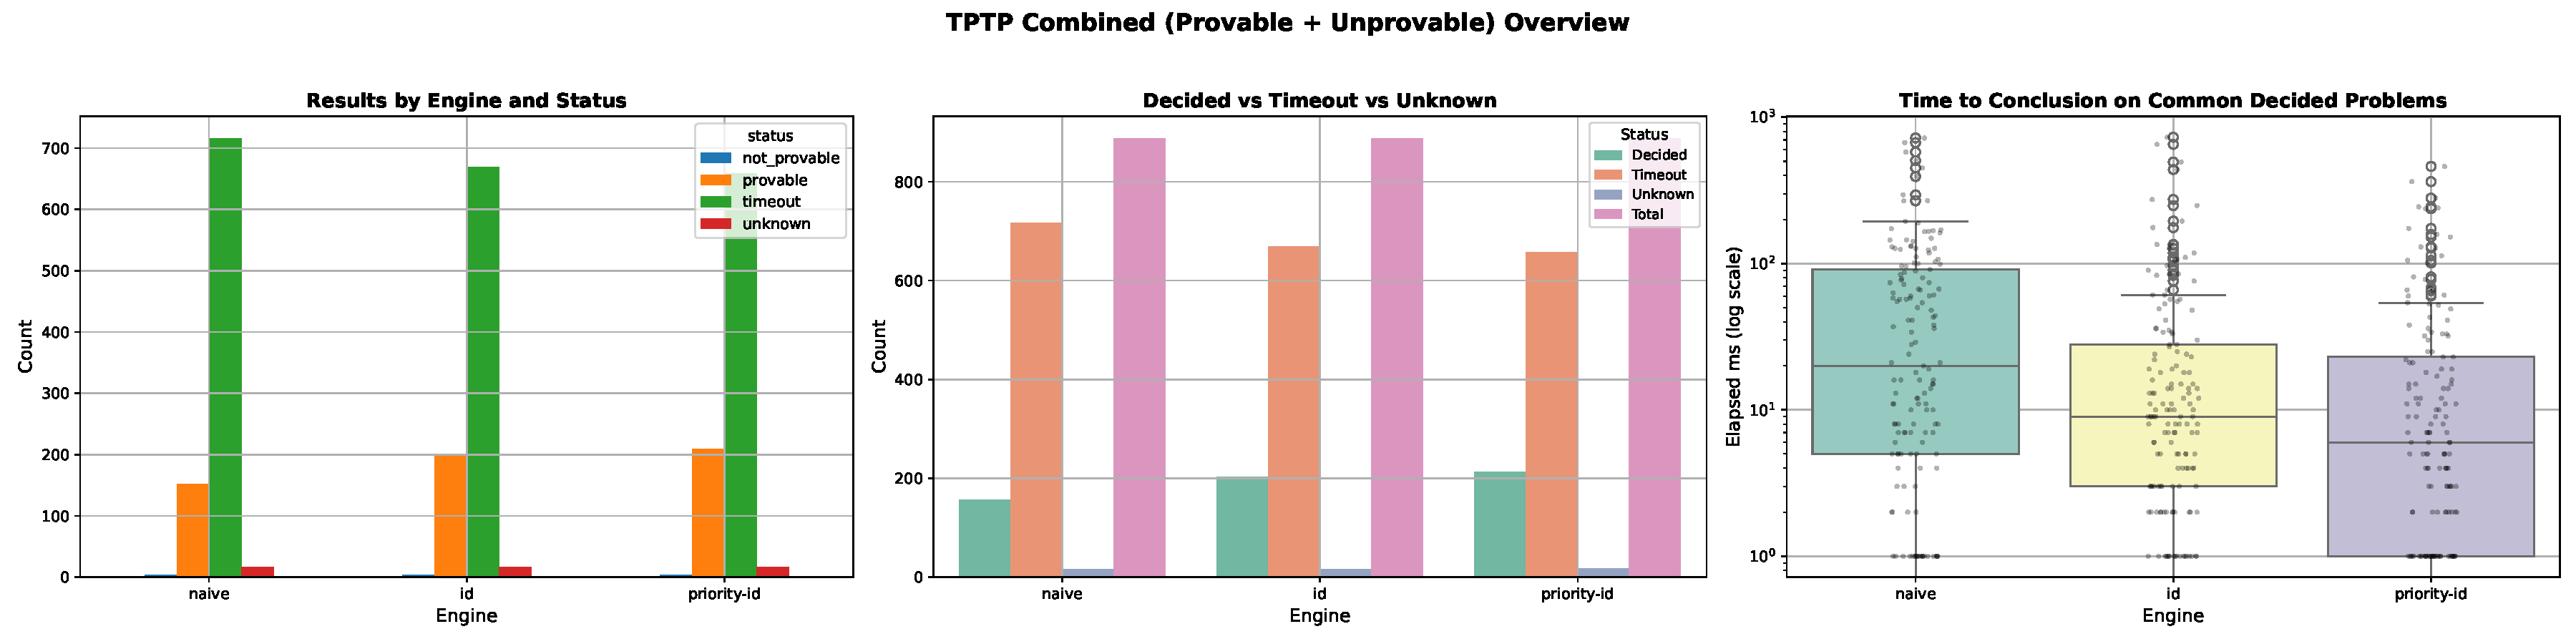
\includegraphics[width=\linewidth]{figures/tptp_combined_overview.pdf}
  \caption{TPTP combined dataset (888 problems): outcome counts by engine
    (left), decided vs.\ timeout vs.\ unknown breakdown (centre), and
    time to conclusion on commonly decided problems, log scale (right).}
  \label{fig:tptp-overview}
\end{figure}

\begin{figure}[h]
  \centering
  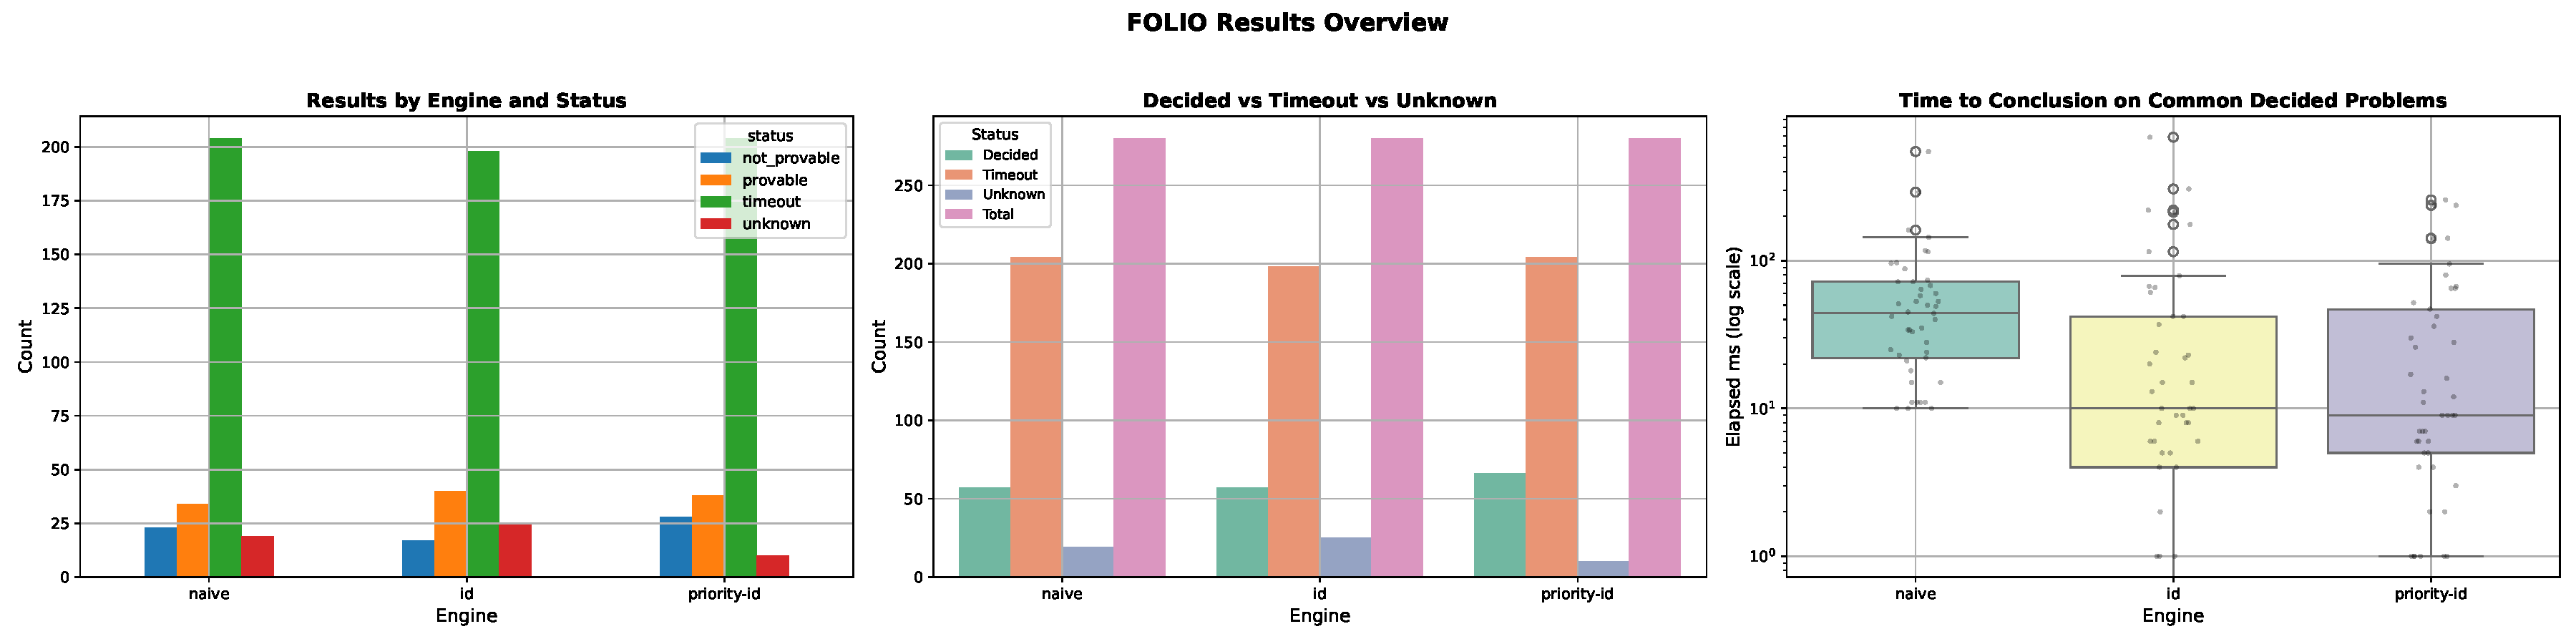
\includegraphics[width=\linewidth]{figures/folio_overview.pdf}
  \caption{FOLIO validation set (280 problems): same layout as
    Fig.~\ref{fig:tptp-overview}.}
  \label{fig:folio-overview}
\end{figure}

\begin{figure}[h]
  \centering
  \includegraphics[width=\linewidth]{figures/ai_generated_overview.pdf}
  \caption{Synthetic dataset (202 problems): same layout as
    Fig.~\ref{fig:tptp-overview}.}
  \label{fig:ai-overview}
\end{figure}

On the TPTP benchmark (Figure~\ref{fig:tptp-overview}), \texttt{naive}
decides 156 problems, \texttt{id} decides 203 ($+30\,\%$), and
\texttt{priority-id} decides 213 ($+37\,\%$ over \texttt{naive}). All
additional solves come from the provable subset; the four
counter-satisfiable decisions are shared by all three engines. The
log-scale timing panel shows that \texttt{id} and \texttt{priority-id}
not only solve problems \texttt{naive} cannot reach, but also solve the
shared problems faster on average, reflecting fewer wasted steps in
dead-end branches.

The FOLIO results (Figure~\ref{fig:folio-overview}) reveal a different
pattern. \texttt{naive} and \texttt{id} both decide 57 problems, but with
a shifted composition: \texttt{naive} returns 34~\textit{Provable} and
23~\textit{NotProvable}, while \texttt{id} returns 40~\textit{Provable}
and 17~\textit{NotProvable}. These are not the same problems. \texttt{id}
finds 11 proofs that \texttt{naive} timed out on, but loses 5 proofs that
\texttt{naive} found: iterative deepening's repeated restarts exhaust
the step budget before those branches close. Simultaneously, \texttt{id}
converts 6 of \texttt{naive}'s \textit{NotProvable} decisions to
\textit{Unknown}: the restarts prevent the search from fully exhausting
those spaces, so problems \texttt{naive} certified as unprovable become
undecided under \texttt{id}. The net result is a coincidental wash at 57
decided problems. \texttt{priority-id} resolves this trade-off by spending
fewer steps per iteration on unproductive branches. It decides 66
problems (38~\textit{Provable} and 28~\textit{NotProvable}), converting
11 of \texttt{id}'s \textit{Unknown} and \textit{Timeout} outcomes to
\textit{NotProvable} (the more disciplined step budget allows those
search spaces to be fully exhausted), and reducing \textit{Unknown} from
25 to 10.

On the synthetic dataset (Figure~\ref{fig:ai-overview}), \texttt{naive}
decides 26 problems, \texttt{id} decides 39 ($+50\,\%$ over
\texttt{naive}), and \texttt{priority-id} decides 42 ($+62\,\%$ over
\texttt{naive}). The tier breakdown
(Figure~\ref{fig:synthetic-tier}, Table~\ref{tab:synthetic-tier}) shows
where these gains arise. On medium-tier problems \texttt{naive} decides
10 of 60, \texttt{id} decides 19, and \texttt{priority-id} decides 20.
On hard-tier problems \texttt{naive} decides none, while \texttt{id} and
\texttt{priority-id} decide 3 and 5 respectively. No engine decides any
expert-tier problem. The gains are concentrated in implication-chain and
syllogism families; all 43 transitivity-chain problems are unsolved by
every engine: every invocation times out, as the repeated-reuse proof
strategy required by those problems does not terminate within the
1{,}000\,ms wall-clock limit.
Figure~\ref{fig:synthetic-depth} plots solve rate against chain depth for
implication-chain problems, confirming that \texttt{naive}'s solve rate
collapses beyond depth~4 while \texttt{id} and \texttt{priority-id}
maintain non-zero solve rates into the hard tier. This is the controlled
signature of F2: the naive DFS descends into distractor-quantifier chains
at every step, making chain depth the dominant cost factor, while
iterative deepening recovers the short proofs that DFS bypasses. All
three engines agree on all four \textit{NotProvable} decisions.

\begin{figure}[h]
  \centering
  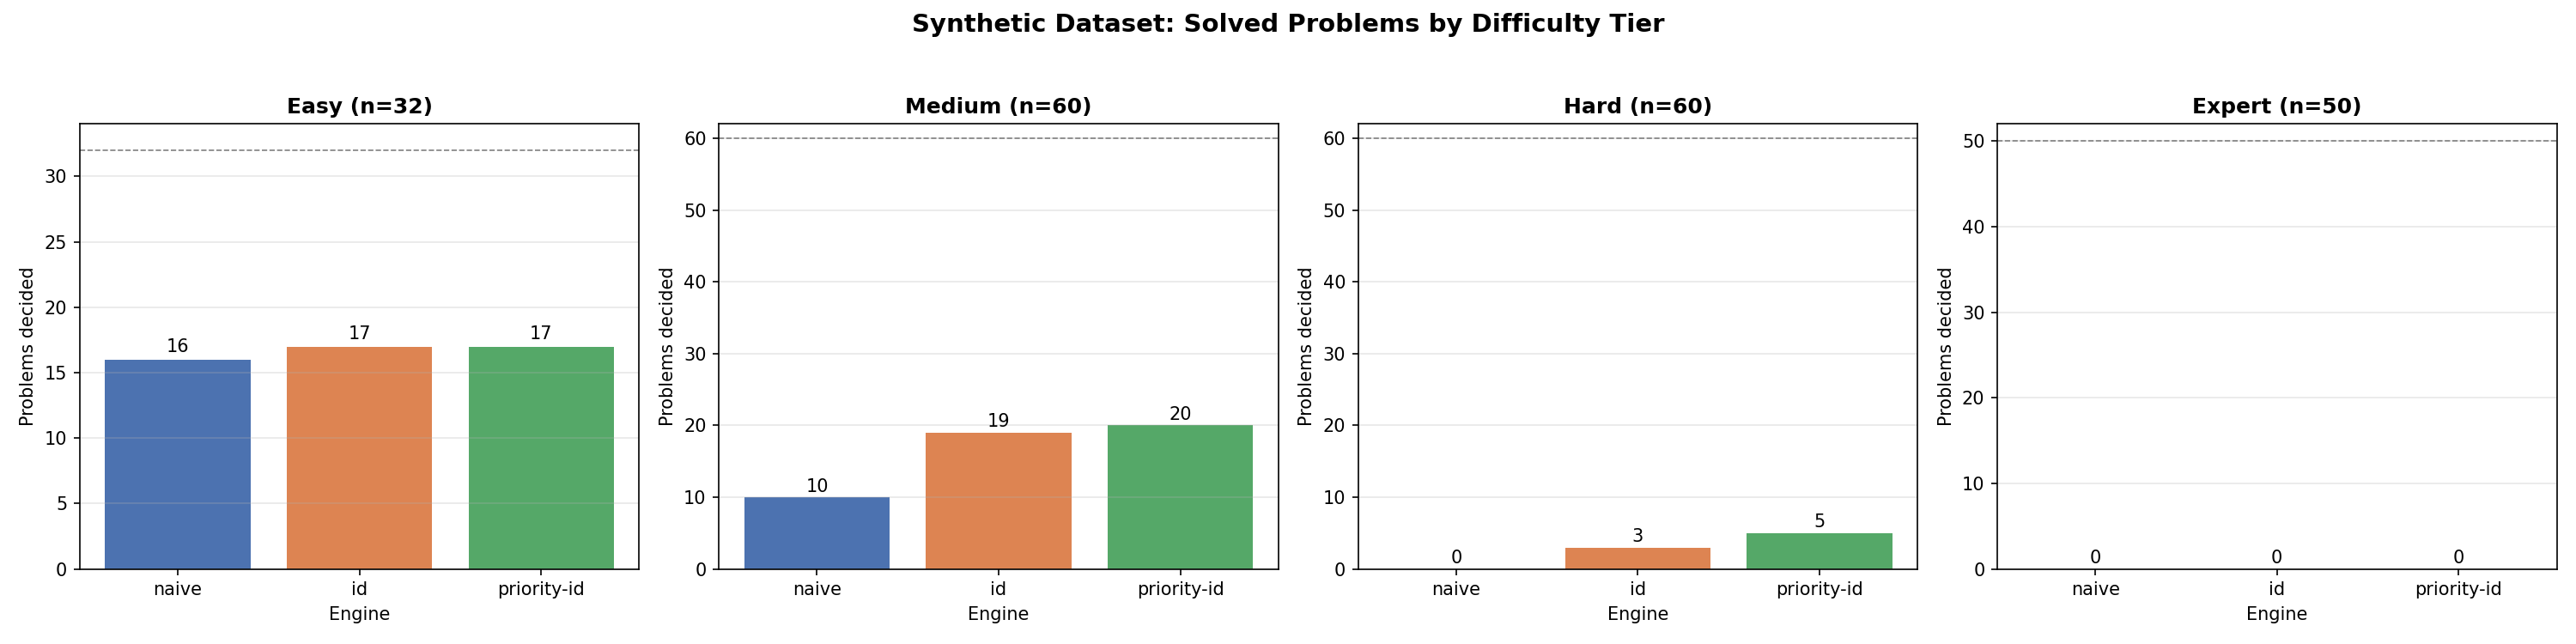
\includegraphics[width=\linewidth]{figures/ai_generated_tier_breakdown.pdf}
  \caption{Synthetic dataset (202 problems): decided problems per engine
    at each difficulty tier. The dashed line marks the total number of
    problems in that tier.}
  \label{fig:synthetic-tier}
\end{figure}

\begin{figure}[h]
  \centering
  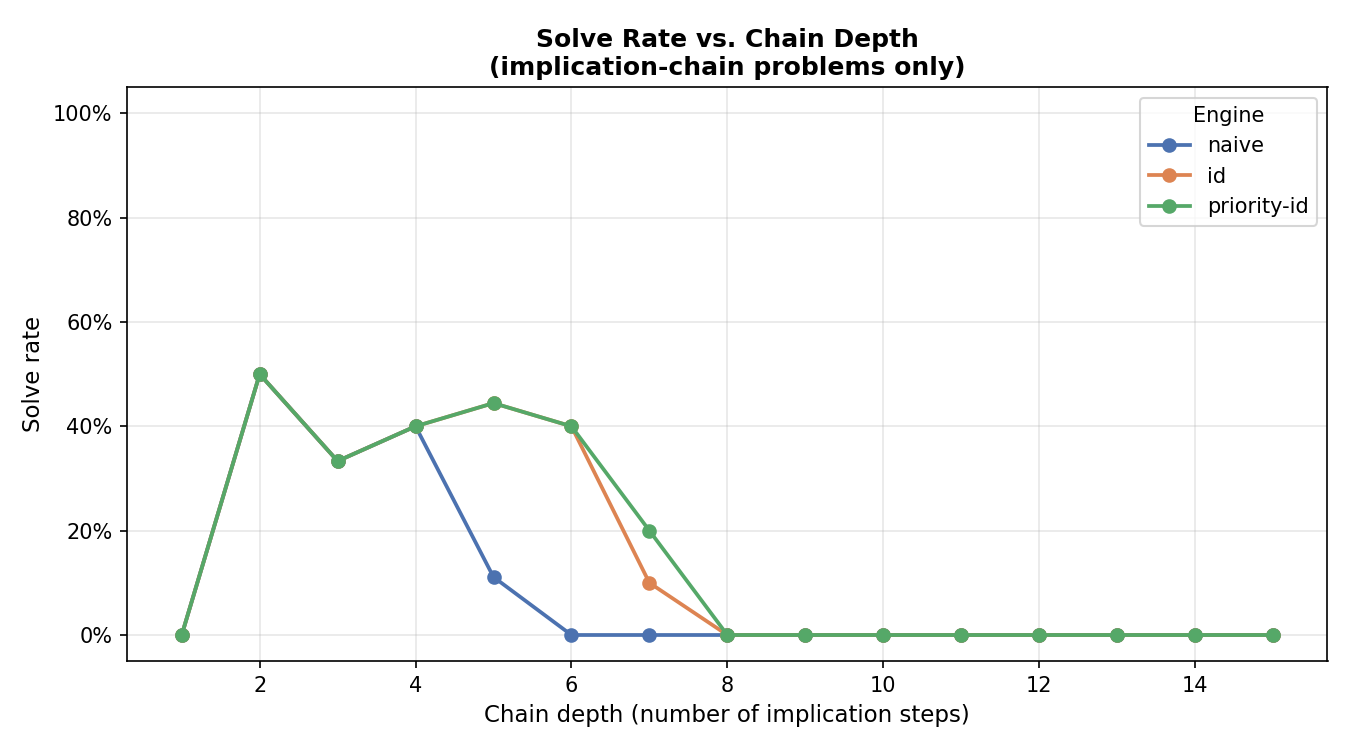
\includegraphics[width=0.85\linewidth]{figures/ai_generated_depth_solve_rate.pdf}
  \caption{Solve rate vs.\ chain depth for implication-chain problems.
    Each point is the fraction of problems at that depth decided by the
    engine; depth is the number of $\forall L$ steps required.}
  \label{fig:synthetic-depth}
\end{figure}

Across all datasets the two refinements are consistently additive.
Iterative deepening provides the larger gain on TPTP and synthetic
problems, where shallow proofs exist but are blocked by deep quantifier
instantiation. The priority schedule drives the net improvement on FOLIO,
where its more disciplined use of the step budget converts undecided
problems into definitive outcomes. Per-dataset breakdowns by outcome type
are given in Appendix~\ref{app:tables}.
